\section{Rigid Body Dynamics}\label{s:Rigid_Body_Dynamics}
This chapter derives all the necessary elements of the the single body dynamics model. The model presented assumes small variability in terrain properties in local regions along both tracks. In addition, since the dynamics of tracked agricultural vehicles do not involve aggressive maneuvers, no lateral or longitudinal weight transfer is modeled. This omits roll and pitch degrees of freedom to allow a planar model of a skid-steered tractor with uniform pressure distributions under each track to be used. To derive the single body model, the tractor is the only rigid body considered. The diagram in \ref{fig:Top_View_Diagram_South_Pole_Traverse} reduces to the free body diagram in Fig. \ref{fig:Single_Body_Free_Body_Diagram} where the inertial coordinates $X, Y$, tractor body fixed coordinates $x, y$, and forces are defined. The vehicle body dynamics are then given by
\begin{equation}\label{eq:RSBD_GBSDX}
    \dot v_x = v_y\dot\theta + \frac{1}{m_T}\Big(F_R + F_L - R_R - R_L - R_{SD} \Big)
\end{equation}
\begin{equation}
    \dot v_y = -v_x\dot\theta + \frac{1}{m_T}\Big(R_{lLF} + R_{lLR} + R_{lRF} + R_{lRR} \Big)
\end{equation}
\begin{equation}
    \ddot\theta = \frac{1}{J_T} \Bigg( \frac{b}{2}F_R - \frac{b}{2}F_L - \frac{b}{2}R_R + \frac{b}{2}R_L + \frac{l}{4}R_{lLF} - \frac{l}{4}R_{lLR} + \frac{l}{4}R_{lRF} - \frac{l}{4}R_{lRR} \Bigg)
\end{equation}
\begin{equation}
    \ddot\varphi_R = \frac{1}{J_S}\Big(\tau_R - F_Rr - \zeta\dot\varphi_R\Big)
\end{equation}
\begin{equation}\label{eq:RSBD_WBSDL}
    \ddot\varphi_L = \frac{1}{J_S}\Big(\tau_L - F_Lr - \zeta\dot\varphi_L\Big)
\end{equation}
\begin{figure}[tb]
    \centering
    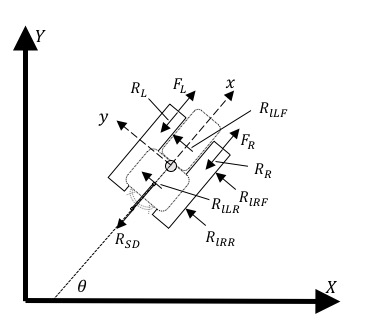
\includegraphics[width = 4in]{Single_Body_Free_Body_Diagram}
    \caption{Free body diagram of the the single body tractor model}
    \label{fig:Single_Body_Free_Body_Diagram}
\end{figure}
where $v_x$, $v_y$, $\dot\theta$, $\dot\varphi_R$ and $\dot\varphi_L$  are the tractor states denoting longitudinal and lateral velocity, the yaw rate, and driver speeds of the right and left tracks respectively. Absolute positions are derived from body-fixed coordinates by
\begin{equation}
      \dot X = v_x\cos\theta - v_y\sin\theta
\end{equation}
\begin{equation}
      \dot Y = v_y\cos\theta + v_x\sin\theta
\end{equation}    
Traction forces of the left and right tracks are denoted as $F_L$ and $F_R$. Track resistance forces are denoted as $R$. $R_L$ and $R_R$ refer to the longitudinal resistance forces on the left and right tracks. $R_{lLF}$, $R_{lLR}$, $R_{lRF}$, and $R_{lRR}$ are the lateral resistance forces on the tracks during turning on the front of the left, the rear of the left track, the front of the right track, and the rear of the right track respectively. The tractor mass and moment of inertia about the $Z$ axis are given by $m_T$ and $J_T$. Important vehicle dimensions not shown in the figure are $l$ and $b$ which are the tracks' nominal ground contact length and the center-to-center distance between the tracks.